%%%%%%%%%%%%%%%%%%%%%%%%%%%%%%%%%%%%%%%%%%%%%%%%%%%%%%%%%%
%
% Doctoral Thesis Template @ The University of Manchester
% LaTeX Chapter Template
% Version 1 (23/07/2020)
% Joe Crone
%
% This template is based on:
% The University of Manchester, Presentation of Thesis Policy
% Research Office Graduate Education Team
% June 2017
% http://www.regulations.manchester.ac.uk/pgr-presentation-theses/
%
%%%%%%%%%%%%%%%%%%%%%%%%%%%%%%%%%%%%%%%%%%%%%%%%%%%%%%%%%%
\documentclass[../main.tex]{subfiles}
\begin{document}

% Title
%--------------------------------------------------------
\chapter{CBETA Inverse Compton Source Design}
\label{CBETA_Inverse_Compton_Source_Design} % to reference use \ref{ChapterTemplate}

\begin{figure}
\centering
\includegraphics[width=0.8\textwidth]{Figures/CBETA_Inverse_Compton_Source_Design/CBETABetaTheta.pdf}
\caption{Tuning curves of $\beta^{*}$ against $\theta_{\mathrm{col}}$ for each of the nominal CBETA electron beam energies satisfying the maximal flux across the 0--1\% bandwidth range. Minimised bandwidth solutions in this range have large $\beta$-functions at the IP and small collimation angles $\theta_{\mathrm{col}}$; the maximal bandwidth solutions have small $\beta$-functions and larger collimation angles $\theta_{\mathrm{col}}$.\textcolor{blue}{**THIS SHOULD BE REPLACED BY ONE FROM NEW CODE WITH LESS NOISE**}}
\label{fig:CBETA_beta_theta_parameter_space}
\end{figure}

\begin{table}
\caption{Electron beam parameters envisaged at the CBETA ICS interaction point (IP). The given baseline parameters -- which assume the same $\beta^*$ at the IP -- allow a comparison of flux and bandwidth at different energies. The optimised values beneath those are where we have maximised the flux into a 0.5\% scattered photon bandwidth through a suitable combination of beam spot size and collimation angle.}
\vspace{3mm}
\resizebox{\textwidth}{!}{%
\begin{tabular}{lccccc}
\hline\hline
Parameter & \multicolumn{4}{c}{Quantity} & Unit \\
\hline
Turn number & 1 & 2 & 3 & 4 & \\
Electron kinetic energy, $E_e$ & 42 & 78 & 114 & 150 & MeV\\
Repetition rate, $f$ & \multicolumn{4}{c}{162.5} & MHz\\
Bunch charge, $e N_e$ & \multicolumn{4}{c}{32} & pC \\
Transverse normalised \textit{rms} emittance, $\epsilon_{N}$ & \multicolumn{4}{c}{0.3} & mm-mrad\\
\textit{rms} bunch length, $\Delta \tau$ & \multicolumn{4}{c}{1.0 (3.33)} & mm (ps)\\
Relative energy spread & \multicolumn{4}{c}{$5.0\times 10^{-4}$} & \\
\hline
 & \multicolumn{4}{c}{Baseline parameters} & \\
\hline
$\beta^*$ (at the IP) & \multicolumn{4}{c}{1} & cm\\
Electron bunch spot size, $\sigma_{\mathrm{electron}}$ & 6.01 & 4.42 & 3.65 & 3.19  & \si{\micro\meter} \\
\hline
 & \multicolumn{4}{c}{Optimised for 0.5\% (narrow) bandwidth} & \\
\hline
$\beta^*$ (at the IP) & 3.56 & 6.58 & 9.60 & 12.62 & cm\\
Electron bunch spot size, $\sigma_{\mathrm{electron}}$ & 11.34 & 11.34 & 11.34 & 11.34  & \si{\micro\meter}\\
Collimation angle, $\theta_{\mathrm{col}}$ & 1.533 & 0.830 & 0.569 & 0.433 & mrad\\
\hline\hline
\end{tabular}}
\label{tab:CBETA_Electron_Beam_Design_Parameters}
\end{table}

\begin{table}
\caption{Nd:YAG laser pulse parameters at the CBETA ICS IP.}
\vspace{3mm}
\centering
\begin{tabular}{lcc}
\hline\hline
Parameter & Quantity & Unit \\
\hline
Wavelength, $\lambda_\textrm{laser}$ & 1064 & nm\\
Photon energy, $E_\textrm{laser}$ & 1.17 & eV\\
Pulse energy  & 62 & \si{\micro\joule}\\
Number of photons, N_{\textrm{laser}} & $3.3\times 10^{14}$\\ 
Repetition rate, $f$ & 162.5 & MHz\\
Spot size at the IP, $\sigma_\textrm{laser}$ & 25 & \si{\micro\meter}\\
Crossing angle, $\phi$ & \ang{5} &  \\
Pulse length  & 10 & ps\\
Relative energy spread, $\Delta E_\textrm{laser}/E_\textrm{laser}$ & 6.57$\times 10^{-4}$ &   \\
 % 0.7nm error on 1064nm
 \hline\hline
\end{tabular}
\label{tab:CBETA_Laser_Pulse_Design_Parameters}
\end{table}

\begin{table}
\caption{Anticipated photon output for each of the four electron beam energies in CBETA, taking into account a 5~degree crossing angle. The uncollimated flux varies by around 2\% due to the small effect of the electron spot size; $X < 0.003$ even at 150~MeV. The collimated flux has been optimised for a 0.5\% bandwidth. The number of scattered photons is essentially independent of electron energy for a fixed electron spot size at the IP, and since both the Compton spectrum and the (relative) 0.5\% bandwidth scale together with $\gamma^2$, both the optimised spot size and the predicted collimated fluxes are the same at all electron energies.}
\vspace{3mm}
\resizebox{\textwidth}{!}{%
\begin{tabular}{lccccc}
\hline\hline
 & \multicolumn{4}{c}{Electron Kinetic Energy (MeV)} & \\
 \cline{2-5}
 & 42 & 78 & 114 & 150 & Unit \\
\hline
X-ray peak energy & 32.2 & 109.7 & 233.1 & 402.5 & keV\\
Uncollimated flux & 3.16$\times10^{10}$ & 3.20$\times10^{10}$ & 3.21$\times10^{10}$ & 3.22$\times10^{10}$ & ph/s\\
Spectral density & 9.82$\times10^{5}$ & 2.92$\times10^{5}$ & 1.38$\times10^{5}$ & 8.00$\times10^{4}$ & ph/s eV\\
Average brilliance & 9.23$\times10^{10}$ & 3.19$\times10^{11}$ & 6.81$\times 10^{11}$ & 1.18$\times10^{12}$ & ph/s mm$^{2}$ mrad$^{2}$ 0.1\% bw\\
Peak brilliance & 2.80$\times 10^{15}$ & 1.00$\times 10^{16}$ & 2.18$\times10^{16}$ & 3.80$\times 10^{16}$ & ph/s mm$^{2}$ mrad$^{2}$ 0.1\% bw\\
\hline
 & \multicolumn{4}{c}{0.5\% bandwidth} & \\
\hline
Collimated flux & 2.09$\times 10^{8}$ & 2.09$\times 10^{8}$ & 2.09$\times 10^{8}$ & 2.09$\times 10^{8}$ & ph/s 0.5\% bw \\
\hline\hline
\end{tabular}}
\label{tab:CBETA_Compton_Output}
\end{table}

\begin{figure}[!htb]
\centering
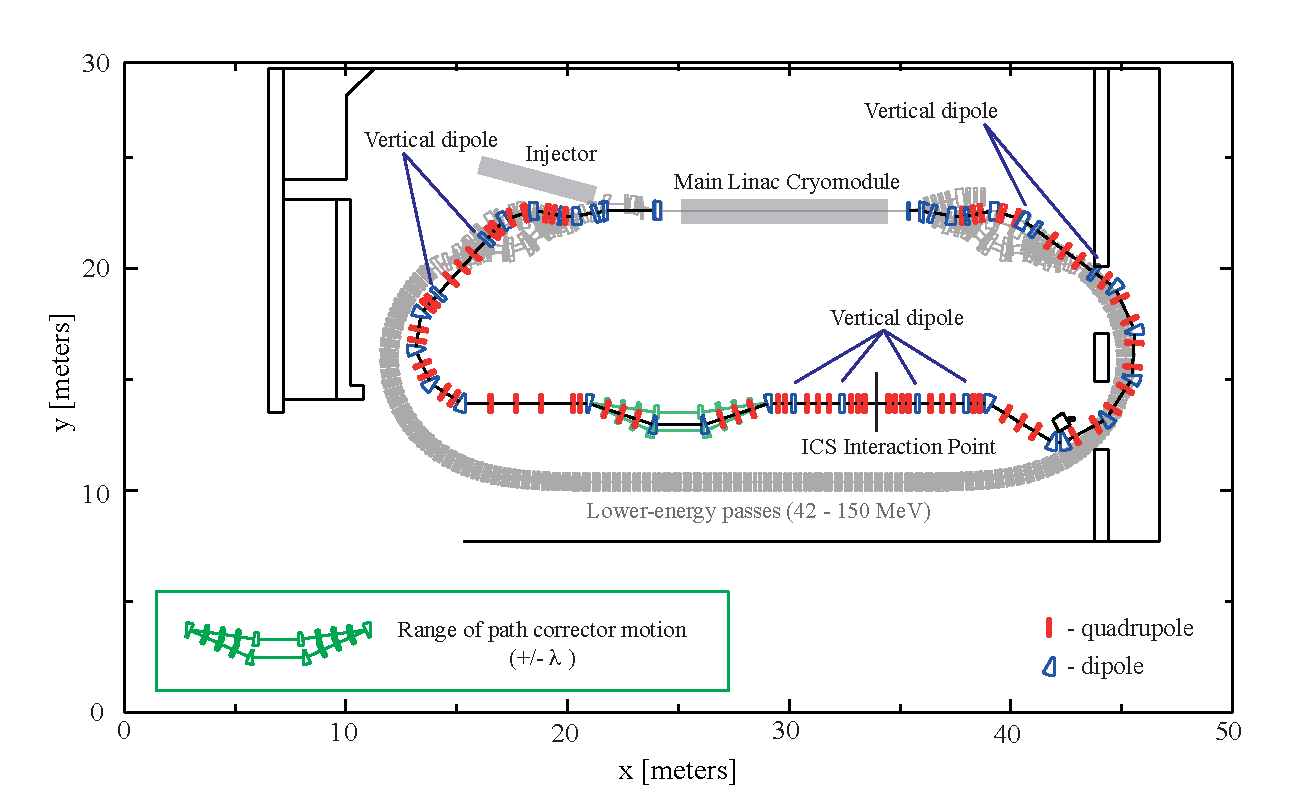
\includegraphics[width=\textwidth]{Figures/CBETA_Inverse_Compton_Source_Design/cbetaicslayout.pdf}
\caption{Layout of the ICS bypass in CBETA; greyed beamline elements are already installed in the existing accelerator. Outer walls and relevant existing infrastructure shown in black.}
\label{fig:CBETA_ICS_Layout}
\end{figure}

\begin{figure}[!htb]
    \centering
    \includegraphics[width=0.8\textwidth]{Figures/CBETA_Inverse_Compton_Source_Design/twissplotx.pdf}
    \includegraphics[width=0.8\textwidth]{Figures/CBETA_Inverse_Compton_Source_Design/twissploty.pdf}
    \caption{Twiss functions in the ICS bypass line, showing the re-matched conditions for different path length configurations $-\lambda_{RF}$, $0$ and $+\lambda_{RF}$. The ICS interaction point (IP) is indicated.}
    \label{fig:CBETA_ICS_Twiss}
\end{figure}

\begin{figure}[!htb]
\centering
\includegraphics[width=0.8\textwidth]{Figures/CBETA_Inverse_Compton_Source_Design/dispplotx.pdf}
\includegraphics[width=0.8\textwidth]{Figures/CBETA_Inverse_Compton_Source_Design/dispplotx.pdf}
\caption{Dispersion functions in the ICS bypass line for the 0.5\% bandwidth case, showing the re-matched conditions for different path length configurations $-\lambda_{RF}$, $0$ and $+\lambda_{RF}$. The ICS interaction point (IP) is indicated.}
\label{fig:CBETA_ICS_dispersion}
\end{figure}

\begin{figure}[!htb]
\centering
\includegraphics[width=0.8\textwidth]{Figures/CBETA_Inverse_Compton_Source_Design/cbetaspectrumplot.pdf}
\caption{Predicted spectral output (flux) from 1064~nm photons colliding head-on with the $E_e =150$~MeV (kinetic energy) electrons in CBETA; this spectrum was generated using the \textsc{ICCS3D} code, and is consistent with calculations using the method of Sun et al. This spectrum has a peak energy of 403.3~keV; using the proposed 5~degree crossing angle, the peak energy is reduced to 402.5~keV and the spectral density is reduced by a factor $\sim$~5.}
\label{fig:CBETA_ICS_Spectra}
\end{figure}

\begin{figure}[!htb]
\centering
\includegraphics[width=0.8\textwidth]{Figures/CBETA_Inverse_Compton_Source_Design/CBETAICSSpectra.pdf}
\caption{Predicted spectra output (flux) from 1064~nm photons colliding head-on with the $E_{e}=150$~MeV electrons accelerated in CBETA. This is a comparison of the \textsc{ICCS3D} code (blue) against the \textsc{SUN1D} semi-analytic code (orange). The \textsc{ICCS3D} spectra uses a tracked distribution of which 1000 particles are sampled, this sampling results in a lower total energy of $E_{e}=150.44$~MeV, hence the lower peak energy.  The spectrum is broadened by the effect of emittance in both planes in \textsc{ICCS3D} in comparison to the 1D emittance model of C. Sun's model/. \textcolor{blue}{**WHY IS THE PEAK ENERGY DIFFERENT**}}
\label{fig:CBETA_ICS_Spectra_Comparison}
\end{figure}

\begin{figure}[!htb]
\centering
\includegraphics[width=0.8\textwidth]{Figures/CBETA_Inverse_Compton_Source_Design/150MeVBenchmarkSpectra.pdf}
\caption{Comparison of predicted spectral output from 1064~nm photons colliding head-on with $E_{Tot}=150$~MeV electrons from CBETA. The emittance is minimised in the $y$ direction ($\epsilon_{ny} = 0.003$~mm-mrad, 100 times smaller than the actual value) in order to benchmark the \textsc{SUN1D} (blue) and \textsc{ICCS3D} (orange) codes. The spectra have identical shapes however the \textsc{SUN1D} spectra has a higher peak amplitude \textcolor{blue}{**WHY**}}
\label{fig:CBETA_Benchmarking_Spectra}
\end{figure}

\begin{figure}[!htb]
\centering
\includegraphics[width=0.8\textwidth]{Figures/CBETA_Inverse_Compton_Source_Design/spring8bl10fluxplot.pdf}
\caption{Comparison of CBETA predicted flux (here flux in a 0.1\% bandwidth to allow comparison with conventional calculations of undulator flux) at the four discrete operating energies given in Table~\ref{tab:compton_output} \textcolor{blue}{**CORRECT ONCE THE TABLES ARE IN**} with the output from a typical high-energy undulator. The undulator shown is the SPRING-8 BL10XU insertion device~\cite{spring8beamlines} assuming an \textit{rms} phase error of 5~degrees. Whilst this undulator is not designed to deliver good output at high harmonic number, it offers a useful guide to possible 3rd-generation source output in the 100~keV to 500~keV range. the measured flux at 30~keV and 61~keV for this beamline is also shown~\cite{spring8beamlines}. We predict that CBETA flux at 402~keV (150~MeV electron energy) exceeds that from 3rd-generation sources.}
\label{fig:ICS_vs_SPRING8_Undulator_Flux}
\end{figure}

\begin{figure}[!htb]
\centering
\includegraphics[width=0.8\textwidth]{Figures/CBETA_Inverse_Compton_Source_Design/spring8bl10brillianceplot.pdf}
\caption{Comparison of CBETA predicted brilliance at the four discrete operating energies given in Table~\ref{tab:compton_output}  \textcolor{blue}{**CORRECT ONCE THE TABLES ARE IN**} with the output from a typical high-energy undulator. The undulator shown is the SPRING-8 BL10XU insertion device~\cite{spring8beamlines} assuming an \textit{rms} phase error of 5~degrees. We predict that CBETA brilliance at 402~keV (150~MeV electron kinetic energy) exceeds that from 3rd-generation sources.}
\label{fig:ICS_vs_SPRING8_Undulator_Brilliance}
\end{figure}

\begin{figure}[!htb]
\centering
\includegraphics[width=0.8\textwidth]{Figures/CBETA_Inverse_Compton_Source_Design/sourcefluxcomparison.pdf}
\caption{On-sample measured fluxes from APS, ESRF-EBS, PETRA-III, and SPRING-8 for which information has been published~\cite{apsbeamlines,esrfbeamlines,petraiiibeamlines,spring8beamlines}. This is compared with the predicted CBETA outputs at the 4 discrete photon energies from 32 to 402~keV, and the predicted flux obtained by scaling the CBETA electron energy to 300~MeV (1600~keV photons) and 600~MeV (6360~keV photons). Whilst 3rd-generation sources are superior to ICS sources up to photon energies around 300~keV, they do not produce useable flux above 400~keV.}
\label{fig:ICS_Undulator_Comparison}
\end{figure}

\end{document}